\section{Job Search with Correlated Wage Draws}
\begin{frame}{Job Search with Correlated wage draws -  Set up}
    We let 
    \begin{itemize}
        \item $(W_t)_{t\ge 0}$ is \textcolor{blue}{P-Markov} and take values from $W\subset \mathbb{R}_+$, $W$ is nonempty.
        \item $\varphi$ is the stationary distribution of $P$, i.e., $\varphi = \varphi P$
        \item $\varphi$ has finite mean, so $\int w\,\varphi(dw)<\infty$
        \item Constant discount factor $\beta\in(0,1)$
        \item $\Sigma$ be the set of Borel measurable policy $\sigma: W\to \{0,1\}$
         \item $L_1(\varphi):= L^1(W,\mathcal{B}, \varphi)$ be all Borel measurable function $f:W\to \mathbb{R}$ with $\int|f|\,d\varphi<\infty$
    \end{itemize}
\end{frame}

\begin{frame}{Comparison}
\textbf{For IID draws}, with $e(w) :=\frac{w}{1-\beta}$
\begin{align*}
    T_\sigma v &= \underbrace{[\sigma e+(1-\sigma)c]}_{=:r_\sigma} + \textcolor{blue}{\underbrace{(1-\sigma)\beta \mathbb{E}v}_{=:K_\sigma v}}\\
    &= r_\sigma + \textcolor{blue}{K_\sigma v}
\end{align*}
\textbf{For Correlated wage draws}
\begin{align*}
    T_\sigma v &= \underbrace{[\sigma e+(1-\sigma)c]}_{=:r_\sigma} + \textcolor{blue}{\underbrace{(1-\sigma)\beta P}_{:=\beta P_\sigma}v}\\
    &= r_\sigma +\textcolor{blue}{\beta P_\sigma v}
\end{align*}
\end{frame}
\begin{frame}{Exercise 4.1.11}
Prove that $T_\sigma$ is an order-preserving self-map on $L_1(\varphi)$.
\begin{proof}
    First, we prove that $T_\sigma$ is a self-map on $L_1(\varphi)$, i.e.,
    $$
    v\in L_1(\varphi)\implies r_\sigma +\beta P_\sigma v\in L_1(\varphi)
    $$
    In particular, we need to show $Pv\in L_1(\varphi)$, i.e., $Pv$ is Borel measurable and
    $$
    \int_{W}\left|\int_{W'} v(w')\, P(w, dw')\right|\,\varphi(dw)<\infty
    $$
\end{proof}
\end{frame}

\begin{frame}{Exercise 4.1.11 cont.}
    \begin{proof}
        $Pv$ is Borel measurable by the property of stochastic kernel. And we have
        \begin{align*}
            \int_{W}\left|\int_{W'} v(w')\, P(w, dw')\right|\,\varphi(dw)&\le \int_{W}\int_{W'}|v(w')|\, P(w,dw')\, \varphi(dw)\tag{Jensen}\\
            &= \int_{W'}\int_W|v(w')|\varphi(dw)P(w,dw')\tag{Tonelli}\\
            &= \int_{W'}|v(w')|\textcolor{blue}{\int_W \varphi(dw)P(w,dw')}\tag{stationary}\\
            &= \int_{W'}|v(w')|\,\textcolor{blue}{\varphi(dw')} <\infty\tag{$\in L_1(\varphi)$}
        \end{align*}
    At last, order preserving is from the property of Markov operator.
    \end{proof}
\end{frame}


\begin{frame}{Value space}
Let $L_1(\varphi)$ paired with almost-everywhere order be the value space,
\begin{itemize}
    \item Banach lattice
    \item \textcolor{blue}{Dedekind complete}
\end{itemize}
\end{frame}

\begin{frame}{Policy operators}
\begin{align*}
    T_\sigma v &= \underbrace{[\sigma e+(1-\sigma)c]}_{=:r_\sigma} + \textcolor{blue}{\underbrace{(1-\sigma)\beta P}_{:=\beta P_\sigma}v}\\
    &= r_\sigma +\textcolor{blue}{\beta P_\sigma v}
\end{align*}
\begin{itemize}
    \item order-preserving self-map on $L_1(\varphi)$
    \item affine
    \item $\beta P_\sigma  \le \beta P$ and $\rho(\beta P) =\beta<1$
\end{itemize}
\end{frame}

\begin{frame}{ADP representation}
The ADP $(L_1(\varphi), \mathbb{T}_{JSM})$ is
    \begin{itemize}
        \item regular
        \item well-posed
    \end{itemize}
with similar proofs from the IID case.   
\end{frame}

\begin{frame}{Optimality}
\begin{figure}
    \centering
    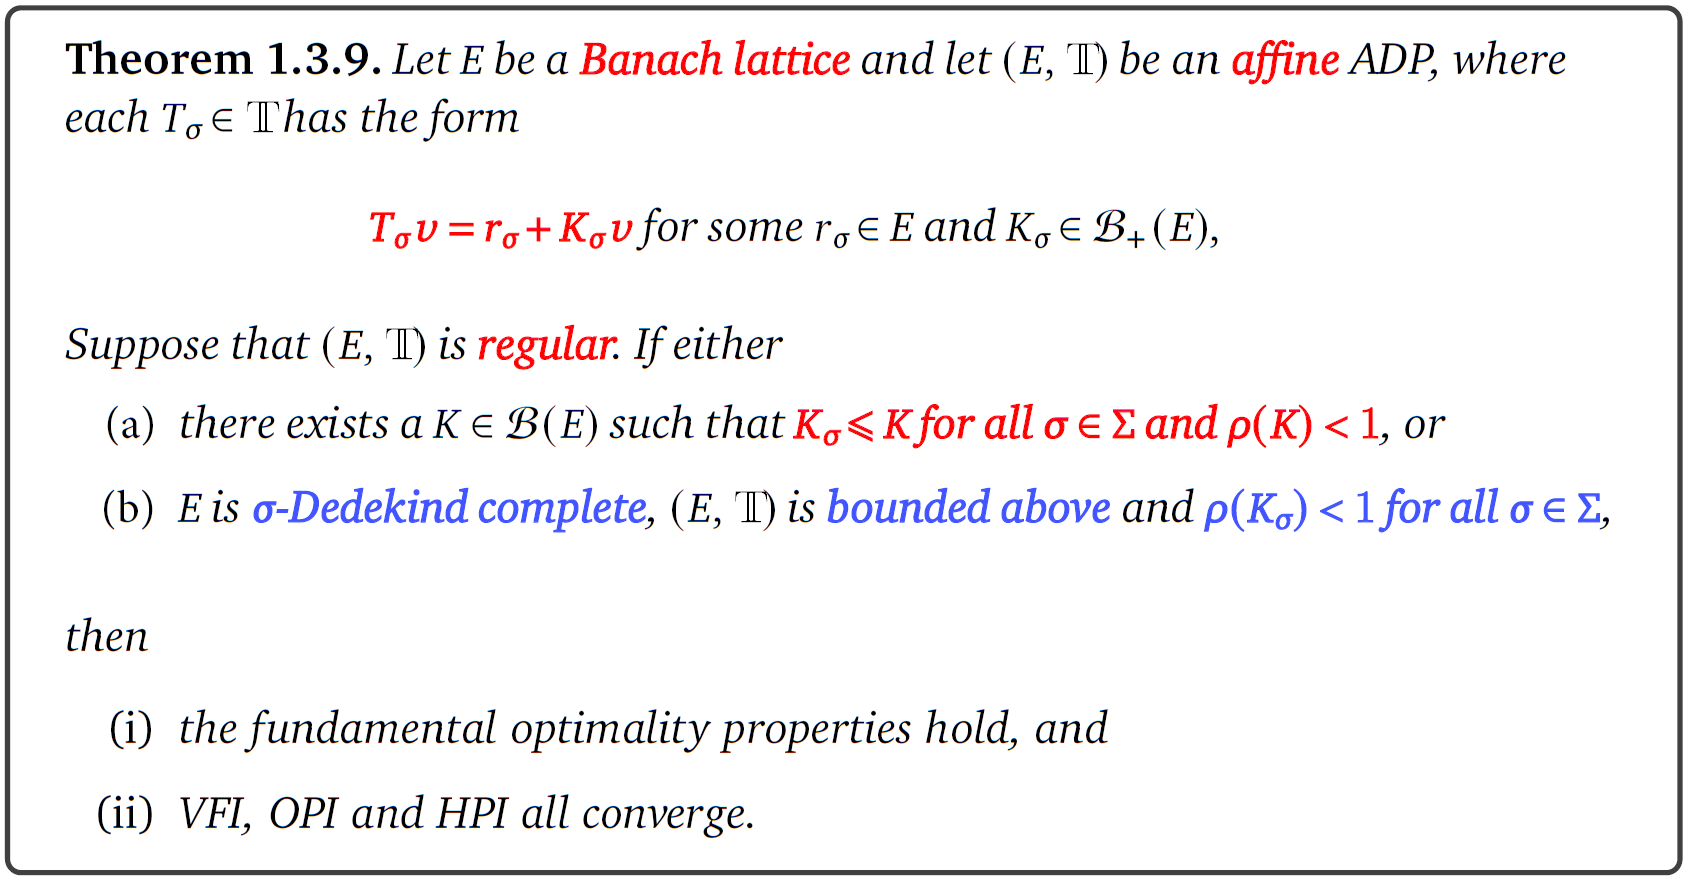
\includegraphics[width=0.9\linewidth]{Dynamic Programming/DP2/Chapter 4/Section 4.1.1. Job Search/thm139new.png}
\end{figure}
\end{frame}

\begin{frame}{Exercise 4.1.15}
Let $\bar v:= (I-\beta P)^{-1}(e+c)$ and $V:= \{v\in L_1(\varphi): 0\le v\le \bar v\}$. Show that, for all $\sigma \in\Sigma$, we have $v_\sigma \le \bar v$ and $T_\sigma V\subset V$ 
\begin{proof}
    We have $T_\sigma \bar v = r_\sigma +\beta P_\sigma \bar v$. By definition, $\bar v = (e+c) + \beta P\bar v$. We know $e+c\ge r_\sigma$, $\beta P\bar v\ge \beta P_\sigma \bar v$ for all $\sigma\in\Sigma$. Hence, We have
    $$
    T_\sigma \bar v\le \bar v
    $$
    By global stability and order preserving, $T_\sigma$ is (strongly) order stable. Hence, we have
    $$
    v_\sigma \le \bar v
    $$
    Moreover $T_\sigma 0 = r_\sigma \ge 0$, hence $T_\sigma V\subset V$.
\end{proof}
\end{frame}
\begin{frame}{Remark: The ADP is bounded above}
We say the ADP is bounded above if there exists a $u\in V$ with $T_\sigma u\precsim u$ for all $T_\sigma\in\mathbb{T}$. From the previous proof, we show that $T_\sigma \bar v\le \bar v$ for all $\sigma \in \Sigma$. This proves that the ADP is bounded above.Hence, we can also use the second line in Theorem 1.3.9
\end{frame}

\begin{frame}{Exercise 4.1.13}
    Show that every policy operator $T_\sigma$ is order continuous on $L_1(\varphi)$.
    \begin{proof}
        See Zaanen (2012). Every positive operator on $L^p$ is order continuous. 
    \end{proof}
\end{frame}

\begin{frame}{Reducing the value space}
We have $V:= \{v\in L_1(\varphi): 0\le v\le \bar v\}$
\begin{itemize}
    \item $V$ is an order interval and Dedekind complete, hence \textcolor{red}{chain complete}
\end{itemize}
We also have the policy operator $T_\sigma$
\begin{itemize}
    \item order preserving self-map on $V$
    \item globally stable hence \textcolor{red}{strongly order stable}
    \item \textcolor{red}{order continuous}
\end{itemize}
For the ADP $(V,\mathbb{T}_{JSM})$
\begin{itemize}
    \item \textcolor{red}{regular}
    \item \textcolor{red}{well-posed}
\end{itemize}
\end{frame}

\begin{frame}{Optimality on the reduced value space (ex4.1.15)}
    \begin{figure}
        \centering
        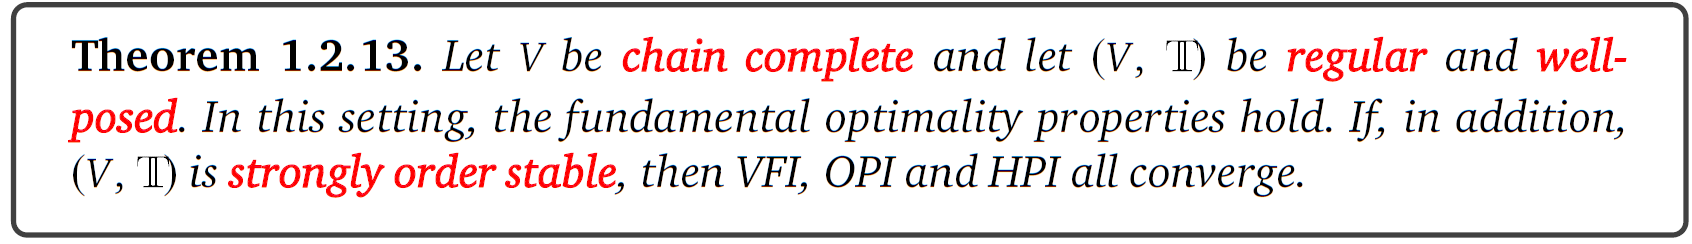
\includegraphics[width=1\linewidth]{Dynamic Programming/DP2/Chapter 4/Section 4.1.1. Job Search/thm1213new.png}
        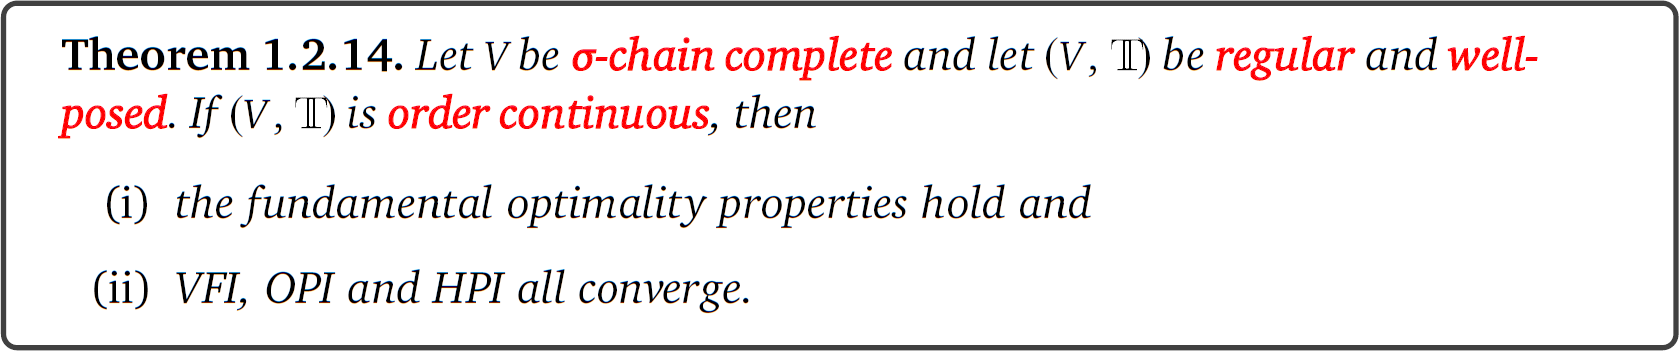
\includegraphics[width=1\linewidth]{Dynamic Programming/DP2/Chapter 4/Section 4.1.1. Job Search/thm1214new.png}
    \end{figure}
\end{frame}

\begin{frame}{Optimality on the reduced value space}
\begin{figure}
    \centering
    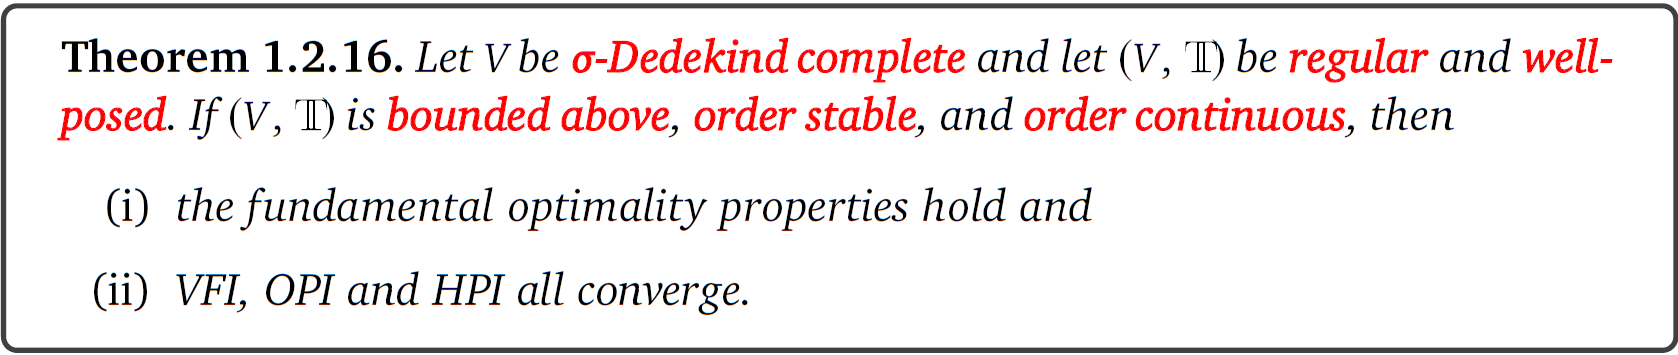
\includegraphics[width=1\linewidth]{Dynamic Programming/DP2/Chapter 4/Section 4.1.1. Job Search/thm1216.png}
\end{figure}    
\end{frame}

\begin{frame}{Exercise 4.1.17}
    Show that if $W$ is finite, the HPI converges in finitely many steps.
    \begin{proof}
        $W$ is finite $\implies \Sigma$ is finite $\implies \mathbb{T}_{JSM}$ is finite. Use Theorem 1.2.12
    \end{proof}
    \begin{figure}
        \centering
        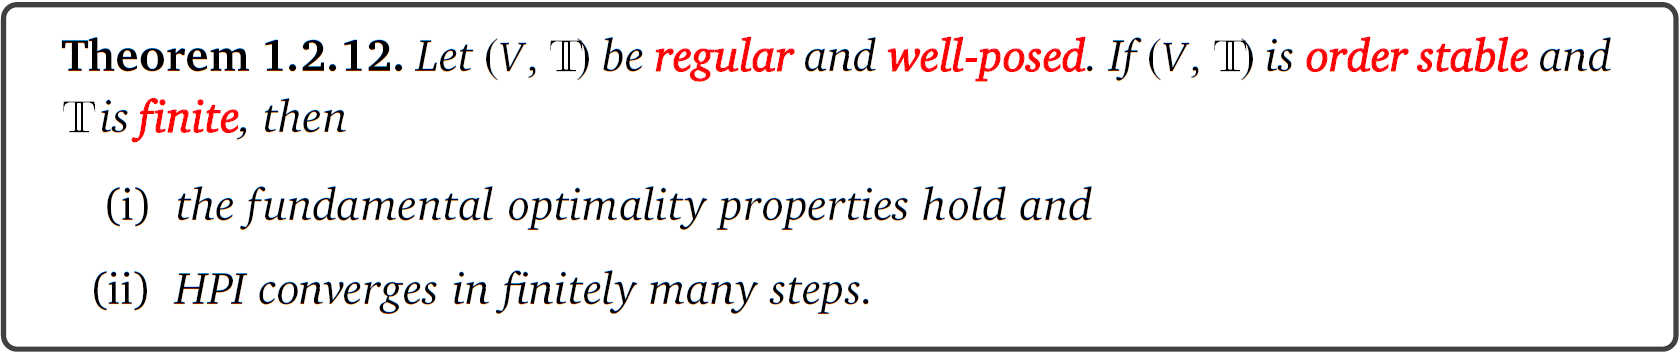
\includegraphics[width=1\linewidth]{Dynamic Programming/DP2/Chapter 4/Section 4.1.1. Job Search/thm1212.png}
    \end{figure}
\end{frame}